\documentclass[14pt]{beamer}
\title[JPL:Java:01]{JPL :: While ... Loops}
\author[TS]{TalentSprint}
\institute[L\&D]{Licensed To Skill}
\date{Version 1.0.4}
\usefonttheme{serif}
\usecolortheme{orchid}
\usepackage{bookman}
\usepackage{hyperref}
\usepackage[font={scriptsize,bf}]{caption}
\usepackage[T1]{fontenc}
\usepackage{color}
\usepackage{graphicx}
\usepackage{listings}
\graphicspath{{../../Images/}}
\usepackage{tikz}
\usepackage{color}
\beamertemplateballitem
\usebackgroundtemplate{
\includegraphics[width=\paperwidth]{TS-XP-Logo.jpg}}
\lstset{language=Java,numbers=left, numberstyle=\tiny, basicstyle=\footnotesize, numbersep=10pt, showstringspaces=false, breaklines=true,keepspaces=true, columns=flexible}
\begin{document}

\begin{frame}
  \titlepage
\end{frame}

\begin{frame}{Learning Objectives}
By the end of this presentation, you will be able to:
  \begin{itemize}
  \item Learn the concept of looping in solutions to problems

  \item Use while loop and do...while loop in Java code.

  \end{itemize}
\end{frame}


\begin{frame}{While...Loops}
 The smiley wants to reach step-5 from bottom
\begin{figure}[H]
\begin{center}
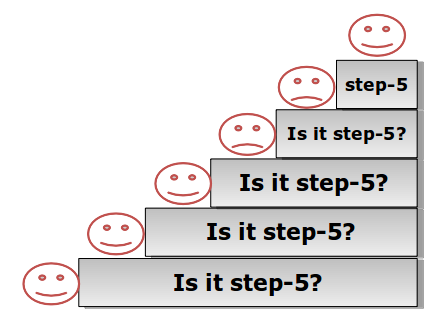
\includegraphics[scale=.4]{smiley.png}
\end{center}
\end{figure}
\end{frame}


\begin{frame}{While...Loops}
\begin{figure}[H]
\begin{center}
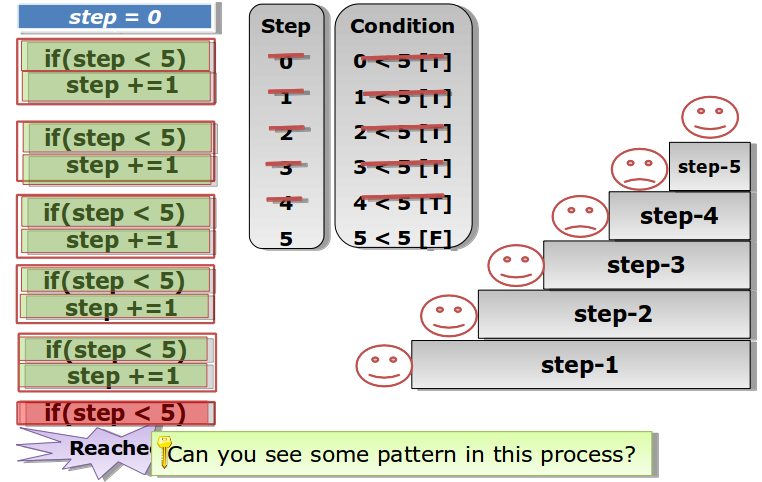
\includegraphics[scale=.4]{while-smiley.png}
\end{center}
\end{figure}
\end{frame}

\begin{frame}{While...Loops}
\begin{figure}[H]
\begin{center}
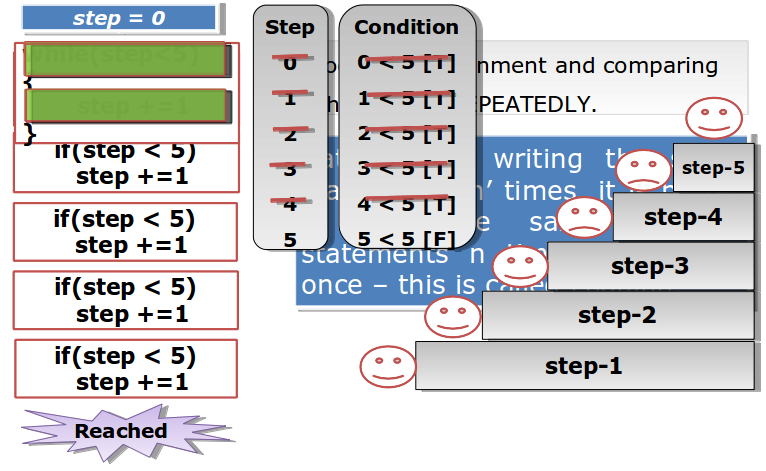
\includegraphics[scale=.4]{while-loop-smiley.png}
\end{center}
\end{figure}
\end{frame}

\begin{frame}{While...Loops}
 To find largest of 'n' numbers
 

 \begin{minipage}{5cm}
  \colorbox{gray}{4, 9, 2, -27, 34, 26, 45, 64, 58, 12, 96, ..., n}
 \end{minipage}
 
\hspace{5cm}$\uparrow$

\hspace{1cm}\begin{minipage}{5cm}
  \colorbox{cyan}{Now, which is the largest number?}
 \end{minipage}
 \begin{block}{How about the following approach:}
 \small
Read first number. Call it largest\_so\_far. 

Read second number into next.

\lstinline!if (next > largest_so_far) largest_so_far = next!

.....

Read 'n'th number into next.

\lstinline!if (next > largest_so_far) largest_so_far = next!

    print largest\_so\_far

 \end{block}
What if n is a big number !!!
\end{frame}

\begin{frame}[fragile]{While...Loops}
 \lstinline!largest = Integer.parseInt(args[0]);!
 
 \lstinline!next = Integer.parseInt(args[1]);!
 
 \begin{lstlisting}[numbers=none]
while(count < args.length){
    if(next > largest)
        largest = next
    next = Integer.parseInt(args[count]);
    count++;
}                 
 \end{lstlisting}
\end{frame}

\begin{frame}[fragile]{While...Loops}
 \begin{block}{Method 1: Java Code}
  \begin{lstlisting}[numbers=none]
public class LargestNumberMany {
    public static void main(String[] args) {
        int next, largestSoFar, count = 0;
        largestSoFar = Integer.parseInt(args[count]);
        count ++;
        while (count < args.length) {
            next = Integer.parseInt(args[count]);
            count ++;
            if (next > largestSoFar)
                largestSoFar = next;
        }
        System.out.println("Largest: " + largestSoFar);
    }
}
  \end{lstlisting}

 \end{block}

\end{frame}

\begin{frame}[fragile]{While...Loops}
 \begin{block}{`While' Statement}
 The `\lstinline!while!' statement is a control flow looping statement that allows the code to be executed repeatedly based on a given Boolean condition. The `\lstinline!while!' statement can be thought of as a repeating `\lstinline!if!' statement. 
 \end{block}
\end{frame}
 
 \begin{frame}[fragile]{While...Loops}
 \begin{minipage}{5cm}
  \begin{block}{Syntax}
   \begin{lstlisting}[numbers=none]
  while (expression) { 
      statement(s);
  }
   \end{lstlisting}

  \end{block}
 \end{minipage}
 \quad
 \begin{minipage}{4cm}
  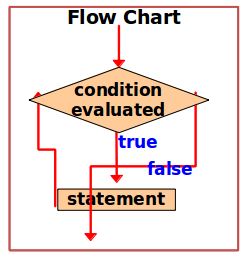
\includegraphics[scale=.4]{while-flow-chart.png}
 \end{minipage}
\end{frame}

\begin{frame}[fragile]{While...Loops}
\begin{minipage}{4cm}
\begin{lstlisting}[numbers=none]
  do {
      step += 1;
  } while (step < 5);  
 \end{lstlisting}
 \end{minipage}
 \quad
 \begin{minipage}{5cm}
 \begin{figure}[H]
 \begin{center}
  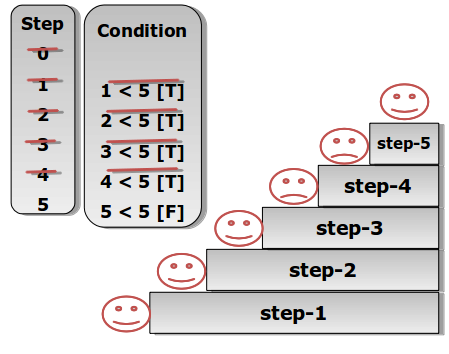
\includegraphics[scale=.4]{while-loop-iteration.png}
 \end{center}
 \end{figure}
  \end{minipage}
\end{frame}

\begin{frame}[fragile]{While...Loops}
 \begin{block}{Method 2: Java Code}
  \begin{lstlisting}[numbers=none]
public class LargestNumberMany2 {
    public static void main(String[] args) {
        int next, largestSoFar, count = 0;
        largestSoFar = Integer.parseInt(args[count++]);
        do {
            next = Integer.parseInt ( args[count++] );
            if (next > largestSoFar)
                largestSoFar = next;
        } while (count < args.length);
        System.out.println("Largest: " + largestSoFar);
    }
}
 \end{lstlisting}
 \end{block}
\end{frame}

\begin{frame}[fragile]{While...Loops}
 `\lstinline!do - while!' Statement
  
  \vspace{1pc}
  The purpose of `\lstinline!do - while!' statement is the same as that of `\lstinline!while!' statement. However, unlike `\lstinline!while!' statement, `\lstinline!do - while!' evaluates its expression at the bottom of the loop. Therefore, the statements within the `\lstinline!do!' block are always executed at least once.
\end{frame}

\begin{frame}[fragile]{While...Loops}
  \begin{minipage}{5cm}
  \begin{block}{Syntax}
   \begin{lstlisting}[numbers=none]
  do { 
      statement(s);
  } while (expression);
   \end{lstlisting}

  \end{block}
 \end{minipage}
 \quad
 \begin{minipage}{4cm}
  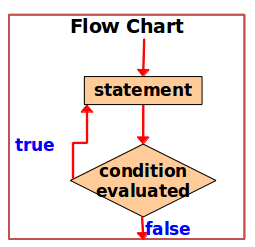
\includegraphics[scale=.4]{do-while-flow-chart.png}
 \end{minipage}
\end{frame}

\begin{frame}[fragile]{While...Loops}
 \begin{enumerate}
  \item Write Java code using \lstinline!while! loop and \lstinline!do... while! loop  for sum of numbers problem. 
  \item Write a program to find out whether a given number is a perfect square or not.
  \item Write a program to find reverse of a given number
  \item Write a program to find sum of digits problem
  \item Write a program to find given number is perfect number or not.
 \end{enumerate}
\end{frame}

\begin{frame}[fragile]{While...Loops}
 \begin{block}{Solution - Exercise 1 (Method 1)}
  \begin{lstlisting}[numbers=none]
public class SumMany {
    public static void main(String[] args) {
        int next, sumSoFar = 0, count = 0;
        while (count < args.length) {
            next = Integer.parseInt(args[count]);
            count ++;
            sumSoFar += next;
        }
        System.out.println("Sum: " + sumSoFar);
    }
}
  \end{lstlisting}
 \end{block}
\end{frame}

\begin{frame}[fragile]{While...Loops}
 \begin{block}{Solution - Exercise 1 (Method 2)}
  \begin{lstlisting}[numbers=none]
public class SumMany2 {
    public static void main(String[] args) {
        int next, sumSoFar = 0, count = 0;
        do {
            next = Integer.parseInt(args[count]);
            count ++;
            sumSoFar += next;
        } while (count < args.length);
        System.out.println("Sum: " + sumSoFar);
    }
}
  \end{lstlisting}
 \end{block}
\end{frame}

\begin{frame}[fragile]{While...Loops}
 \begin{block}{Solution - Exercise 2}
  \begin{lstlisting}[numbers=none]
public class PerfSquare {
    public static void main(String[] args) {
        int i = 1;
        int givenNumber = Integer.parseInt(args[0]);
        while (i < givenNumber) {
            if (i * i == givenNumber) {
                System.out.println(givenNumber + " is perfect square");
                return;
            }
            i++;
        }
        System.out.println(givenNumber + " is not perfect square");
    }
}
  \end{lstlisting}
 \end{block}
\end{frame}




\begin{frame}{While...Loops}
 \begin{figure}[H]
 \begin{center}
   
\includegraphics[scale=.3]{qa.png}   
 \end{center}
  \end{figure}
\end{frame}



\end{document}

